\section{Hebb則と教師なし学習}
\subsection{Hebb則}
神経回路はどのようにして自己組織化するのだろうか.1940年代にカナダの心理学者Donald O. Hebbにより著書"The Organization of Behavior"\cite{Hebb1949-iv} で提案された学習則は「細胞Aが反復的または持続的に細胞Bの発火に関与すると,細胞Aが細胞Bを発火させる効率が向上するような成長過程または代謝変化が一方または両方の細胞に起こる」というものであった.すなわち,発火に時間的相関のある細胞間のシナプス結合を強化するという学習則である.これを\textbf{Hebbの学習則 (Hebbian learning rule)}\index{Hebbのがくしゅうそく (Hebbian learning rule)@Hebbの学習則 (Hebbian learning rule)} あるいは\textbf{Hebb則(Hebb's rule)}\index{Hebbのり(Hebb's rule)@Hebb則(Hebb's rule)} という.Hebb則は (Hebb自身ではなく) Shatzにより"cells that fire together wire together" (共に活動する細胞は共に結合する)と韻を踏みながら短く言い換えられている \cite{Shatz1992-he}.

\subsubsection{Hebb則の導出}
数式でHebb則を表してみよう.$n$個のシナプス前細胞と$m$個の後細胞の発火率をそれぞれ$\mathbf{x}\in \mathbb{R}^n, \mathbf{y}\in \mathbb{R}^m$ とする.前細胞と後細胞間のシナプス結合強度を表す行列を$\mathbf{W}\in \mathbb{R}^{m\times n}$とし,$\mathbf{y}=\mathbf{W}\mathbf{x}$が成り立つとする.このようなモデルを線形ニューロンモデル (Linear neuron model) という.このとき,Hebb則は


\begin{equation}
\tau\frac{d\mathbf{W}}{dt}=\phi(\mathbf{y})\varphi(\mathbf{x})^\top
\end{equation}


として表される.ただし,$\tau$は時定数であり,$\eta\triangleq1/\tau$ は\textbf{学習率 (learning rate)}\index{がくしゅうりつ (learning rate)@学習率 (learning rate)} と呼ばれる学習の速さを決定するパラメータとなる.$\varphi(\cdot)$および$\phi(\cdot)$は,それぞれシナプス前細胞および後細胞の活動量に応じて重みの変化量を決定する関数である.ただし,$\varphi(\cdot), \phi(\cdot)$は基本的に恒等関数に設定される場合が多い.この場合,Hebb則は$
\tau\dfrac{d\mathbf{W}}{dt}=\mathbf{y}\mathbf{x}^\top=(\text{post})\cdot (\text{pre})^\top
$と簡潔に表現される.

このHebb則は数学的に導出されたものではないが,特定の目的関数を神経活動及び重みを変化させて最適化するようなネットワークを構築すれば自然に出現する.このようなネットワークを\textbf{エネルギーベースモデル (energy-based models)}\index{えねるぎーべーすもでる (energy-based models)@エネルギーベースモデル (energy-based models)} といい,次章で扱う.エネルギーベースモデルでは,先にエネルギー関数 (あるいはコスト関数) $\mathcal{E}$ を定義し,その目的関数を最小化するような神経活動 $\mathbf{z}$ および重み行列 $\mathbf{W}$ のダイナミクスをそれぞれ,


\begin{equation}
\frac{d \mathbf{z}}{dt}\propto-\frac{\partial \mathcal{E}}{\partial \mathbf{z}},\ \frac{d \mathbf{W}}{dt}\propto-\frac{\partial \mathcal{E}}{\partial \mathbf{W}}
\end{equation}


として導出する.この手順の逆を行う,すなわち先に神経細胞の活動ダイナミクスを定義し,神経活動で積分することで神経回路のエネルギー関数$\mathcal{E}$を導出し,さらに $\mathcal{E}$ を重み行列で微分することでHebb則が導出できる \cite{Isomura2020-sn}.Hebb則の導出を連続時間線形ニューロンモデル $\dfrac{d\mathbf{y}}{dt}=\mathbf{W}\mathbf{x}$ を例にして考えよう.ここで$\dfrac{\partial\mathcal{E}}{\partial\mathbf{y}}\triangleq-\dfrac{d\mathbf{y}}{dt}$となるようなエネルギー関数 $\mathcal{E}(\mathbf{x}, \mathbf{y}, \mathbf{W})$を仮定すると,


\begin{equation}
\mathcal{E}(\mathbf{x}, \mathbf{y}, \mathbf{W})=-\int \mathbf{W}\mathbf{x}\ d\mathbf{y}=-\mathbf{y}^\top \mathbf{W}\mathbf{x} \in \mathbb{R}
\end{equation}


となる.これをさらに$\mathbf{W}$で微分すると,


\begin{equation}
\dfrac{\partial\mathcal{E}}{\partial\mathbf{W}}=-\mathbf{y}\mathbf{x}^\top\Rightarrow
\frac{d\mathbf{W}}{dt}=-\dfrac{\partial\mathcal{E}}{\partial\mathbf{W}}=\mathbf{y}\mathbf{x}^\top
\end{equation}


となり,Hebb則が導出できる (簡単のため時定数は1とした).
\subsection{Hebb則の安定化とLTP/LTD}
\subsubsection{BCM則}
Hebb則には問題点があり,シナプス結合強度が際限なく増大するか,0に近づくこととなってしまう.これを数式で確認しておこう.前細胞と後細胞がそれぞれ1つの場合を考える.2細胞間の結合強度を$w\ (>0)$ とし,$y=wx$が成り立つとすると,Hebb則は$\dfrac{dw}{dt}=\eta yx=\eta x^2w$となる.この場合,$\eta x^2>1$ なら $\lim_{t\to\infty} w= \infty$, $\eta x^2<1$ なら $\lim_{t\to\infty} w= 0$ となる.当然,生理的にシナプス結合強度が無限大となることはあり得ないが,不安定なほど大きくなってしまう可能性があることに違いはない.このため,Hebb則を安定化させるための修正が必要とされた.

Cooper, Liberman, Ojaらにより頭文字をとって\textbf{CLO則}\index{CLOのり@CLO則} (CLO rule) が提案された \cite{Cooper1979-wz}.その後,Bienenstock, Cooper, Munroらにより提案された学習則は同様に頭文字をとって\textbf{BCM則}\index{BCMのり@BCM則} (BCM rule) と呼ばれている\cite{Bienenstock1982-km} \cite{Cooper2012-ec}.

$\mathbf{x}\in \mathbb{R}^d, \mathbf{w}\in \mathbb{R}^d, y\in \mathbb{R}$とし,単一の出力$y = \mathbf{w}^\top \mathbf{x}=\mathbf{x}^\top \mathbf{w}$を持つ線形ニューロンを仮定する.重みの更新則は次のようにする.


\begin{equation}
\frac{d\mathbf{w}}{dt} = \eta_w \mathbf{x} \phi(y, \theta_m)
\end{equation}


ここで関数$\phi$は$\phi(y, \theta_m)=y(y-\theta_m)$などとする.また$\theta_m\triangleq\mathbb{E}[y^2]$は閾値を決定するパラメータ,\textbf{修正閾値(modification threshold)}\index{しゅうせいいきち(modification threshold)@修正閾値(modification threshold)} であり,


\begin{equation}
\frac{d\theta_m}{dt} = \eta_{\theta} \left(y^2-\theta_m\right)
\end{equation}


として更新される.

ToDo: 詳細
\lstinputlisting[language=julia]{./text/local-learning-rule/pca-hebbian-learning/002.jl}
\lstinputlisting[language=julia]{./text/local-learning-rule/pca-hebbian-learning/003.jl}
\lstinputlisting[language=julia]{./text/local-learning-rule/pca-hebbian-learning/004.jl}
\begin{figure}[ht]
	\centering
	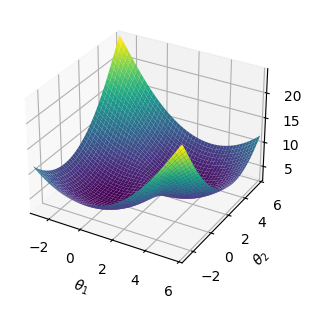
\includegraphics[scale=0.8, max width=\linewidth]{./fig/bayesian-brain/mcmc/cell004.png}
	\caption{cell004.png}
	\label{cell004.png}
\end{figure}
\subsubsection{Hebb則の生理的機序}
ここでHebb則およびBCM則の生理的基盤について触れておこう.
LTPの実験的発見 \cite{Bliss1973-vj} \cite{Dudek1992-nz}

ToDo:実験的発見のsurvey
\subsubsection{Oja則}
Hebb則を安定化させる別のアプローチとして,結合強度を正規化するという手法が考えられる.BCM則と同様に$\mathbf{x}\in \mathbb{R}^d, \mathbf{w}\in \mathbb{R}^d, y\in \mathbb{R}$とし,単一の出力$y = \mathbf{w}^\top \mathbf{x}=\mathbf{x}^\top \mathbf{w}$を持つ線形ニューロンを仮定する.$\eta$を学習率とすると,$\mathbf{w}\leftarrow\dfrac{\mathbf{w}+\eta \mathbf{x}y}{\|\mathbf{w}+\eta \mathbf{x}y\|}$とすれば正規化できる.ここで,$f(\eta)\triangleq\dfrac{\mathbf{w}+\eta \mathbf{x}y}{\|\mathbf{w}+\eta \mathbf{x}y\|}$とし,$\eta=0$においてTaylor展開を行うと,


\begin{align}
f(\eta)&\approx f(0) + \eta \left.\frac{df(\eta^*)}{d\eta^*}\right|_{\eta^*=0} + \mathcal{O}(\eta^2)\\
&=\frac{\mathbf{w}}{\|\mathbf{w}\|} + \eta \left(\frac{\mathbf{x}y}{\|\mathbf{w}\|}-\frac{y^2\mathbf{w}}{\|\mathbf{w}\|^3}\right)+ \mathcal{O}(\eta^2)
\end{align}


ここで$\|\mathbf{w}\|=1$として,1次近似すれば$f(\eta)\approx \mathbf{w} + \eta \left(\mathbf{x}y-y^2 \mathbf{w}\right)$となる.重みの変化が連続的であるとすると,


\begin{equation}
\frac{d\mathbf{w}}{dt} = \eta \left(\mathbf{x}y-y^2 \mathbf{w}\right)
\end{equation}


として重みの更新則が得られる.これを\textbf{Oja則 (Oja's rule)}\index{Ojaのり (Oja's rule)@Oja則 (Oja's rule)} と呼ぶ \cite{Oja1982-yd}.こうして得られた学習則において$\|\mathbf{w}\|\to 1$となることを確認しよう.


\begin{equation}
\frac{d\|\mathbf{w}\|^2}{dt}=2\mathbf{w}^\top\frac{d\mathbf{w}}{dt}= 2\eta y^2\left(1-\|\mathbf{w}\|^2\right)
\end{equation}


より,$\dfrac{d\|\mathbf{w}\|^2}{dt}=0$のとき,$\|\mathbf{w}\|= 1$となる.
\subsubsection{恒常的可塑性}
Oja則は更新時の即時的な正規化から導出されたものであるが,恒常的可塑性 (synaptic scaling)により安定化しているという説がある\cite{Turrigiano2008-lm}\cite{Yee2017-fb}.しかし,この過程は遅すぎるため,Hebb則の不安定化を安定化するに至らない\cite{Zenke2017-el}

ToDo:恒常的可塑性の詳細

Johansen, Joshua P., Lorenzo Diaz-Mataix, Hiroki Hamanaka, Takaaki Ozawa, Edgar Ycu, Jenny Koivumaa, Ashwani Kumar, et al. 2014. “Hebbian and Neuromodulatory Mechanisms Interact to Trigger Associative Memory Formation.” Proceedings of the National Academy of Sciences 111 (51): E5584–92.
\subsection{Hebb則と主成分分析}
Oja則を用いることで\textbf{主成分分析(Principal component analysis; PCA)}\index{しゅせいぶんぶんせき(Principal component analysis; PCA)@主成分分析(Principal component analysis; PCA)} という処理をニューラルネットワークにおいて実現できる.主成分分析とは-

ToDo:主成分分析の説明
\lstinputlisting[language=julia]{./text/local-learning-rule/pca-hebbian-learning/009.jl}
\lstinputlisting[language=julia]{./text/local-learning-rule/pca-hebbian-learning/010.jl}
\lstinputlisting[language=julia]{./text/local-learning-rule/pca-hebbian-learning/011.jl}
\begin{figure}[ht]
	\centering
	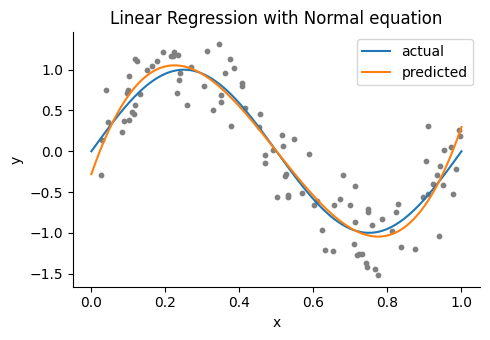
\includegraphics[scale=0.8, max width=\linewidth]{./fig/introduction/linear-regression/cell011.png}
	\caption{cell011.png}
	\label{cell011.png}
\end{figure}
\subsubsection{Oja則によるPCAの実行}
ここでOja則が主成分分析を実行できることを示す.重みの変化量の期待値を取る.


\begin{align}
\frac{d\mathbf{w}}{dt} &= \eta \left(\mathbf{x}y - y^2 \mathbf{w}\right)=\eta \left(\mathbf{x}\mathbf{x}^\top \mathbf{w} - \left[\mathbf{w}^\top \mathbf{x}\mathbf{x}^\top \mathbf{w}\right] \mathbf{w}\right)\\
\mathbb{E}\left[\frac{d\mathbf{w}}{dt}\right] &= \eta \left(\mathbf{C} \mathbf{w} - \left[\mathbf{w}^\top \mathbf{C} \mathbf{w}\right] \mathbf{w}\right)
\end{align}


$\mathbf{C}\triangleq\mathbb{E}[\mathbf{x}\mathbf{x}^\top]\in \mathbb{R}^{d\times d}$とする.$\mathbf{x}$の平均が0の場合,$\mathbf{C}$は分散共分散行列である.$\mathbb{E}\left[\dfrac{d\mathbf{w}}{dt}\right]=0$となる$\mathbf{w}$が収束する固定点(fixed point)では次の式が成り立つ.


\begin{equation}
\mathbf{C}\mathbf{w} = \lambda \mathbf{w}
\end{equation}


これは固有値問題であり,$\lambda\triangleq\mathbf{w}^\top \mathbf{C} \mathbf{w}$は固有値,$\mathbf{w}$は固有ベクトル(eigen vector)になる.

ここでサンプルサイズを$n$とし,$\mathbf{X} \in \mathbb{R}^{d\times n}, \mathbf{y}=\mathbf{X}^\top\mathbf{w} \in \mathbb{R}^n$とする.標本平均で近似して$\mathbf{C}\simeq \mathbf{X}\mathbf{X}^\top$とする.この場合,


\begin{align}
\mathbb{E}\left[\frac{d\mathbf{w}}{dt}\right] &\simeq \eta \left(\mathbf{X}\mathbf{X}^\top \mathbf{w} - \left[\mathbf{w}^\top \mathbf{X}\mathbf{X}^\top \mathbf{w}\right] \mathbf{w}\right)\\
&=\eta \left(\mathbf{X}\mathbf{y} - \left[\mathbf{y}^\top\mathbf{y}\right] \mathbf{w}\right)
\end{align}


となる.
\lstinputlisting[language=julia]{./text/local-learning-rule/pca-hebbian-learning/013.jl}
\lstinputlisting[language=julia]{./text/local-learning-rule/pca-hebbian-learning/014.jl}
\begin{figure}[ht]
	\centering
	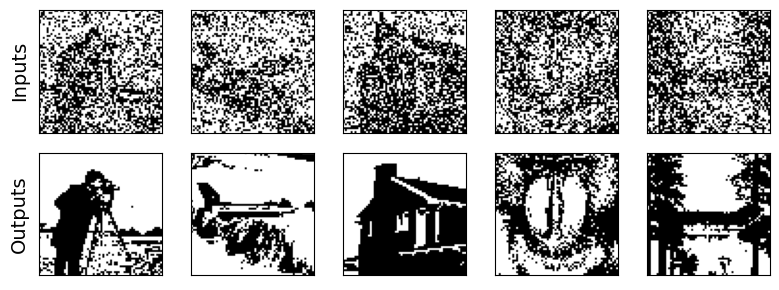
\includegraphics[scale=0.8, max width=\linewidth]{./fig/energy-based-model/hopfield-model/cell014.png}
	\caption{cell014.png}
	\label{cell014.png}
\end{figure}
後のためにOja則においてネットワークが$q$個の複数出力を持つ場合を考えよう.重み行列を$\mathbf{W} \in \mathbb{R}^{q\times d}$, 出力を$\mathbf{y}=\mathbf{W}\mathbf{x} \in \mathbb{R}^{q}, \mathbf{Y}=\mathbf{W}\mathbf{X} \in \mathbb{R}^{q\times n}$とする.この場合の更新則は


\begin{equation}
\frac{d\mathbf{W}}{dt} = \eta \left(\mathbf{y}\mathbf{x}^\top - \mathrm{Diag}\left[\mathbf{y}\mathbf{y}^\top\right] \mathbf{W}\right)
\end{equation}


となる.ただし,$\mathrm{Diag}(\cdot)$は行列の対角成分からなる対角行列を生み出す作用素である.
\subsubsection{Sanger則}
Oja則に複数の出力を持たせた場合であっても,出力が直交しないため,PCAの第1主成分しか求めることができない.\textbf{Sanger則 (Sanger's rule)}\index{Sangerのり (Sanger's rule)@Sanger則 (Sanger's rule)},あるいは\textbf{一般化Hebb則 (generalized Hebbian algorithm; GHA)}\index{いっぱんかHebbのり (generalized Hebbian algorithm; GHA)@一般化Hebb則 (generalized Hebbian algorithm; GHA)} は,Oja則に\textbf{Gram–Schmidtの正規直交化法(Gram–Schmidt orthonormalization)}\index{Gram–Schmidtのせいきちょっこうかほう(Gram–Schmidt orthonormalization)@Gram–Schmidtの正規直交化法(Gram–Schmidt orthonormalization)} を組み合わせた学習則であり,次式で表される.


\begin{equation}
\frac{d\mathbf{W}}{dt} = \eta \left(\mathbf{y}\mathbf{x}^\top - \mathrm{LT}\left[\mathbf{y}\mathbf{y}^\top\right] \mathbf{W}\right)
\end{equation}


$\mathrm{LT}(\cdot)$は行列の対角成分より上側の要素を0にした下三角行列(lower triangular matrix)を作り出す作用素である.Sanger則を用いればPCAの第2主成分以降も求めることができる.
\lstinputlisting[language=julia]{./text/local-learning-rule/pca-hebbian-learning/017.jl}
\lstinputlisting[language=julia]{./text/local-learning-rule/pca-hebbian-learning/018.jl}
\begin{figure}[ht]
	\centering
	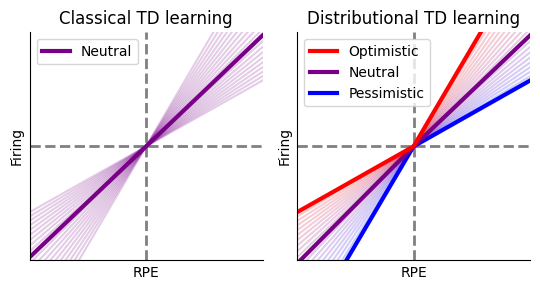
\includegraphics[scale=0.8, max width=\linewidth]{./fig/bayesian-brain/quantile-expectile-regression/cell018.png}
	\caption{cell018.png}
	\label{cell018.png}
\end{figure}
Oja則,Sanger則をまとめて一つの関数にしておこう.\jl{identity()}は恒等関数である.
\lstinputlisting[language=julia]{./text/local-learning-rule/pca-hebbian-learning/020.jl}
\subsection{非線形Hebb学習}
出力$\mathbf{y}$に非線形関数$g(\cdot)$を適用し,$\mathbf{y}\to g(\mathbf{y})$として置き換えることで非線形Hebb学習となる\cite{Oja1997-hr}\cite{Brito2016-mx}. 関数\jl{HebbianPCA}の\jl{func}引数に非線形関数を渡すことで実現できる.

ToDo: 詳細
\subsubsection{非負主成分分析によるグリッドパターンの創発}
内側嗅内皮質(MEC)にある\textbf{グリッド細胞 (grid cells)}\index{ぐりっどさいぼう (grid cells)@グリッド細胞 (grid cells)} は六角形格子状の発火パターンにより自己位置等を符号化するのに貢献している.この発火パターンを生み出すモデルは多数あるが,\textbf{場所細胞(place cells)}\index{ばしょさいぼう(place cells)@場所細胞(place cells)} の発火パターンを\textbf{非負主成分分析(nonnegative principal component analysis)}\index{ひふしゅせいぶんぶんせき(nonnegative principal component analysis)@非負主成分分析(nonnegative principal component analysis)} で次元削減するとグリッド細胞のパターンが生まれるというモデルがある \cite{Dordek2016-ff}.非線形Hebb学習を用いてこのモデルを実装しよう.なお,同様のことは\textbf{非負値行列因子分解 (NMF: nonnegative matrix factorization)}\index{ひふあたいぎょうれついんしぶんかい (NMF: nonnegative matrix factorization)@非負値行列因子分解 (NMF: nonnegative matrix factorization)} でも可能である.
\paragraph{場所細胞の発火パターン}
まず,訓練データとなる場所細胞の発火パターンを人工的に作成する.場所細胞の発火パターンは\textbf{Difference of Gaussians (DoG)}\index{Difference of Gaussians (DoG)} で近似する.DoGは大きさの異なる2つのガウス関数の差分を取った関数であり,画像に適応すればband-passフィルタとして機能する.また,DoGは網膜神経節細胞等の受容野のON中心OFF周辺型受容野のモデルとしても用いられる.受容野中央では活動が大きく,その周辺では活動が抑制される,という特性を持つ.2次元のガウス関数とDoG関数を実装する.
\lstinputlisting[language=julia]{./text/local-learning-rule/pca-hebbian-learning/024.jl}
モデルのパラメータを設定する.
\lstinputlisting[language=julia]{./text/local-learning-rule/pca-hebbian-learning/026.jl}
先にガウス関数とDoG関数がどのような見た目になるか確認しよう.
\lstinputlisting[language=julia]{./text/local-learning-rule/pca-hebbian-learning/028.jl}
\lstinputlisting[language=julia]{./text/local-learning-rule/pca-hebbian-learning/029.jl}
\begin{figure}[ht]
	\centering
	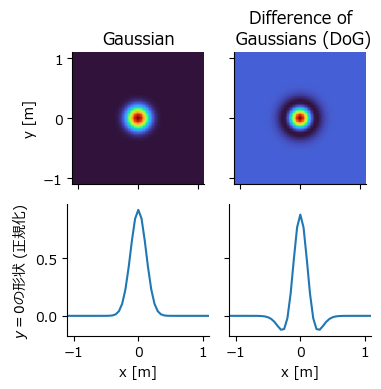
\includegraphics[scale=0.8, max width=\linewidth]{./fig/local-learning-rule/pca-hebbian-learning/cell029.png}
	\caption{cell029.png}
	\label{cell029.png}
\end{figure}
場所細胞の活動パターンを生み出す.それぞれの場所受容野の中心は空間を均等に覆うように作成する (一様分布で生み出してもよい).
\lstinputlisting[language=julia]{./text/local-learning-rule/pca-hebbian-learning/031.jl}
線形PCAの場合
\lstinputlisting[language=julia]{./text/local-learning-rule/pca-hebbian-learning/033.jl}
\lstinputlisting[language=julia]{./text/local-learning-rule/pca-hebbian-learning/034.jl}
\begin{figure}[ht]
	\centering
	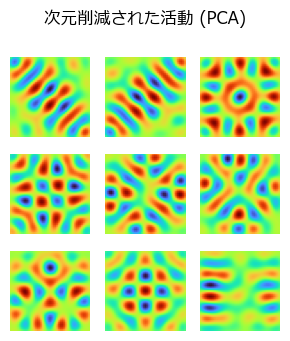
\includegraphics[scale=0.8, max width=\linewidth]{./fig/local-learning-rule/pca-hebbian-learning/cell034.png}
	\caption{cell034.png}
	\label{cell034.png}
\end{figure}
自己相関マップ(autocorrelation map)を確認する.

ToDo: 相関の計算の説明
\lstinputlisting[language=julia]{./text/local-learning-rule/pca-hebbian-learning/036.jl}
\lstinputlisting[language=julia]{./text/local-learning-rule/pca-hebbian-learning/037.jl}
\lstinputlisting[language=julia]{./text/local-learning-rule/pca-hebbian-learning/038.jl}
\begin{figure}[ht]
	\centering
	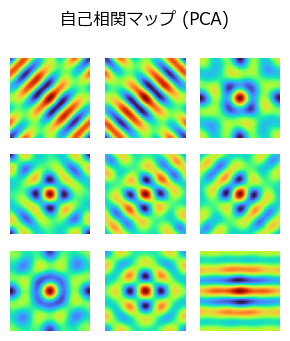
\includegraphics[scale=0.8, max width=\linewidth]{./fig/local-learning-rule/pca-hebbian-learning/cell038.png}
	\caption{cell038.png}
	\label{cell038.png}
\end{figure}
非負PCAの場合
\lstinputlisting[language=julia]{./text/local-learning-rule/pca-hebbian-learning/040.jl}
\lstinputlisting[language=julia]{./text/local-learning-rule/pca-hebbian-learning/041.jl}
\lstinputlisting[language=julia]{./text/local-learning-rule/pca-hebbian-learning/042.jl}
\begin{figure}[ht]
	\centering
	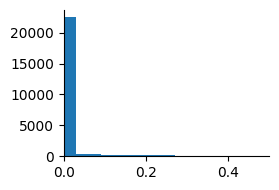
\includegraphics[scale=0.8, max width=\linewidth]{./fig/energy-based-model/sparse-coding/cell042.png}
	\caption{cell042.png}
	\label{cell042.png}
\end{figure}
\lstinputlisting[language=julia]{./text/local-learning-rule/pca-hebbian-learning/043.jl}
\lstinputlisting[language=julia]{./text/local-learning-rule/pca-hebbian-learning/044.jl}
\begin{figure}[ht]
	\centering
	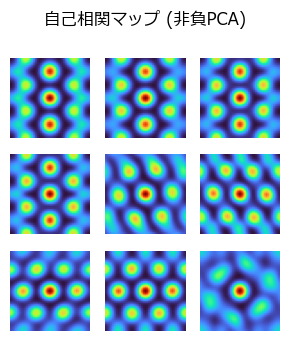
\includegraphics[scale=0.8, max width=\linewidth]{./fig/local-learning-rule/pca-hebbian-learning/cell044.png}
	\caption{cell044.png}
	\label{cell044.png}
\end{figure}
Place cellの受容野をDoGに設定したが,これが無いと格子状の受容野は出現しない.path integrationをRNNで実行する場合も同様.一方で,DoGは場所細胞の受容野としては不適切である.

No Free Lunch from Deep Learning in Neuroscience: A Case Study through Models of the Entorhinal-Hippocampal Circuit 
\url{https://openreview.net/forum?id=mxi1xKzNFrb}

ToDo: 他のgrid cellsのモデルについて
